%package list
\documentclass{article}
\usepackage[top=3cm, bottom=3cm, outer=3cm, inner=3cm]{geometry}
\usepackage{graphicx}
\usepackage{url}
%\usepackage{cite}
\usepackage{hyperref}
\usepackage{array}
\usepackage{multicol}
\newcolumntype{x}[1]{>{\centering\arraybackslash\hspace{0pt}}p{#1}}
\usepackage{natbib}
\usepackage{pdfpages}
\usepackage{multirow}
\usepackage{float}
\usepackage[normalem]{ulem}
\useunder{\uline}{\ul}{}


%%%%%%%%%%%%%%%%%%%%%%%%%%%%%%%%%%%%%%%%%%%%%%%%%%%%%%%%%%%%%%%%%%%%%%%%%%%%
%%%%%%%%%%%%%%%%%%%%%%%%%%%%%%%%%%%%%%%%%%%%%%%%%%%%%%%%%%%%%%%%%%%%%%%%%%%%
\newcommand{\csemail}{vmachacaa@unsa.edu.pe}
\newcommand{\csdocente}{Vicente Machaca Arceda}
\newcommand{\cscurso}{Estructura de Datos y Algoritmos}
\newcommand{\csuniversidad}{Universidad Nacional de San Agustín}
\newcommand{\csescuela}{Maestría en Ciencia de la Computación}
\newcommand{\cspracnr}{01}
\newcommand{\cstema}{--}
%%%%%%%%%%%%%%%%%%%%%%%%%%%%%%%%%%%%%%%%%%%%%%%%%%%%%%%%%%%%%%%%%%%%%%%%%%%%
%%%%%%%%%%%%%%%%%%%%%%%%%%%%%%%%%%%%%%%%%%%%%%%%%%%%%%%%%%%%%%%%%%%%%%%%%%%%


\usepackage[english,spanish]{babel}
\usepackage[utf8]{inputenc}
\AtBeginDocument{\selectlanguage{spanish}}
\renewcommand{\figurename}{Figura}
\renewcommand{\refname}{Referencias}
\renewcommand{\tablename}{Tabla} %esto no funciona cuando se usa babel
\AtBeginDocument{%
	\renewcommand\tablename{Tabla}
}

\usepackage{fancyhdr}
\pagestyle{fancy}
\fancyhf{}
\setlength{\headheight}{30pt}
\renewcommand{\headrulewidth}{1pt}
\renewcommand{\footrulewidth}{1pt}
\fancyhead[L]{\raisebox{-0.2\height}{
\includegraphics[width=3cm]{logo_unsa}}}

\fancyhead[C]{}
\fancyhead[R]{\fontsize{7}{7}\selectfont	\csuniversidad \\ \csescuela \\ \textbf{\cscurso} }
\fancyfoot[L]{MSc. Vicente Machaca}
\fancyfoot[C]{\cscurso}
\fancyfoot[R]{Página \thepage}







\begin{document}
	
	\vspace*{10px}
	
	\begin{center}	
		\fontsize{17}{17} \textbf{ Práctica \cspracnr}
	\end{center}
	%\centerline{\textbf{\underline{\Large Título: Informe de revisión del estado del arte}}}
	%\vspace*{0.5cm}
	

	\begin{table}[h]
		\begin{tabular}{|x{4.7cm}|x{4.8cm}|x{4.8cm}|}
			\hline 
			\textbf{DOCENTE} & \textbf{CARRERA}  & \textbf{CURSO}   \\
			\hline 
			\csdocente & \csescuela & \cscurso    \\
			\hline 
		\end{tabular}
	\end{table}	
	
	
	\begin{table}[h]
		\begin{tabular}{|x{4.7cm}|x{4.8cm}|x{4.8cm}|}
			\hline 
			\textbf{PRÁCTICA} & \textbf{TEMA}  & \textbf{DURACIÓN}   \\
			\hline 
			\cspracnr & \cstema & 3 horas   \\
			\hline 
		\end{tabular}
	\end{table}
	
	
	\section{Datos de los estudiantes}
	\begin{itemize}
		\item Grupo: 3
		\item Integrantes: 
		\begin{itemize}
			\item Lizarraga Mendoza David Jesus
			\item Saenz Mamani Alex Alberto
			\item Huaman Hilari Julissa Zaida
			\item Chara Condori Julio Cesar
			\item Acuña Chavez Melvin
		\end{itemize}		
	\end{itemize}
	
	
	

	
	\section{Ejercicios}\label{sec:ejercicios}
	\begin{enumerate}
		\item Preparación de los datos. Usted debe generar varios conjuntos de datos (archivos .txt ), por
ejemplo va a generar números aleatorios y los va a almacenar en varios archivos. Cada archivo
deberá contener respectivamente 100, 500, 1000, 2000, 3000, ... , 10000, 20000, 30000, ... ,100000
datos.\\
		
		Solución: \\\\
		Se generó 21 archivos txt utilizando el siguiente algoritmo desarrollado en python, ubicado en el siguiente link: \url{https://github.com/julissah/EDA-M/blob/development/GenarateFile/generatefile.py}
		
		\item Implemente los siguientes algoritmos en C++ y Python:\\
		
		Solución:  \\\\
		Se implentó los siguientes algoritmos de ordenamiento, los cuales estan ubicados en el siguiente link \url{https://github.com/julissah/EDA-M/tree/development}:\\
		
		Bubble sort\\
        Counting sort\\
        Heap sort\\
        Insertion sort\\
        Merge sort\\
        Quick sort\\
        Selection sort\\
        
\item Realice comparaciones del tiempo de procesamiento de cada algoritmo por cada lenguaje de programación.
    \begin{enumerate}
        %%%%BUBLE
        \item En la Figura 1, se muestra una comparación del Buble sort y Python. El eje x representa diferentes tamaños de vector a ordenar y el eje y, representa
            el tiempo de procesamiento.\\\\
    
        \begin{figure1}
        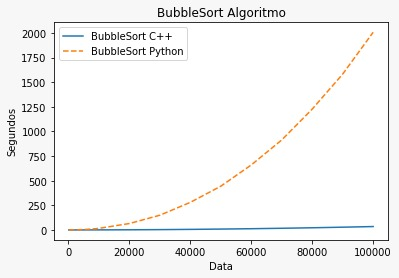
\includegraphics{bubble.jpeg}
        \caption{Figura 1: Comparación de Buble Sort en C++ y Python.}
        \centering
        \end{figure1}\\
        \clearpage
        
        %%%%COUNTING
        \item En la Figura 2, se muestra una comparación del counting sort y Python. El eje x representa diferentes tamaños de vector a ordenar y el eje y, representa
            el tiempo de procesamiento.\\\\
    
        \begin{figure2}
        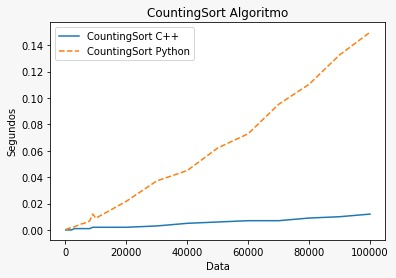
\includegraphics{counting.jpeg}
        \caption{Figura 2: Comparación de Counting Sort en C++ y Python.}
        \centering
        \end{figure2}\\
        \clearpage
        
        %%%%heap
        \item En la Figura 3, se muestra una comparación del heap sort y Python. El eje x representa diferentes tamaños de vector a ordenar y el eje y, representa
            el tiempo de procesamiento.\\\\
    
        \begin{figure3}
        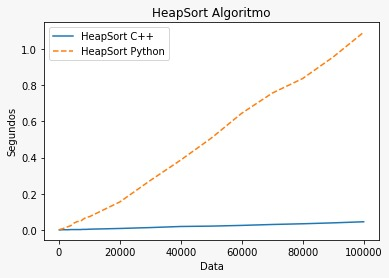
\includegraphics{heap.jpeg}\\
        \caption{Figura 3: Comparación de Heap sort en C++ y Python.}
        \centering
        \end{figure3}\\
        \clearpage
        
        %%%%Insertion sort
        \item En la Figura 4, se muestra una comparación del insertion sort y Python. El eje x representa diferentes tamaños de vector a ordenar y el eje y, representa
            el tiempo de procesamiento.\\\\
    
        \begin{figure4}
        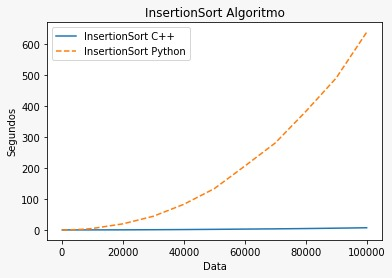
\includegraphics{insertion.jpeg}\\
        \caption{Figura 4: Comparación de Insertion sort en C++ y Python.}
        \centering
        \end{figure4}\\
        \clearpage
        
                %%%%Merge
        \item En la Figura 5, se muestra una comparación del merge sort y Python. El eje x representa diferentes tamaños de vector a ordenar y el eje y, representa
            el tiempo de procesamiento.\\\\
    
        \begin{figure5}
        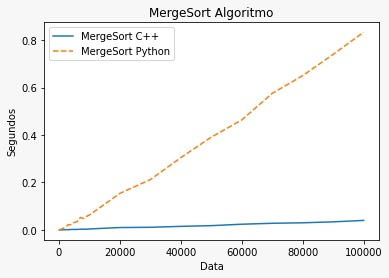
\includegraphics{merge.jpeg}\\
        \caption{Figura 5: Comparación de Merge sort en C++ y Python.}
        \centering
        \end{figure5}\\
        \clearpage
        
                %%%%Quick
        \item En la Figura 6, se muestra una comparación del quick sort y Python. El eje x representa diferentes tamaños de vector a ordenar y el eje y, representa
            el tiempo de procesamiento.\\\\
    
        \begin{figure6}
        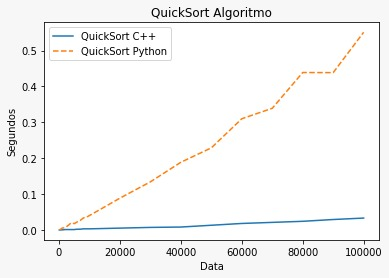
\includegraphics{quick.jpeg}\\
        \caption{Figura 6: Comparación de Quick sort en C++ y Python.}
        \centering
        \end{figure6}\\
        \clearpage
        
                        %%%%c++
        \item Comparación del tiempo de procesamiento de todos los algoritmos implementados en C++. En la Figura 7, se muestra la comparación en C++.\\\\
    
        \begin{figure7}
        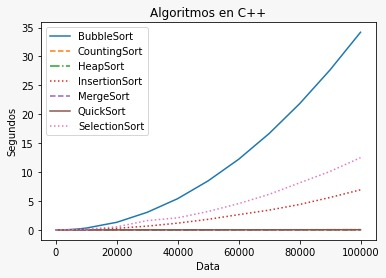
\includegraphics{c++.jpeg}\\
        \caption{Figura 7: Comparación de los algoritmos de ordenamiento en C++.}
        \centering
        \end{figure7}\\
        \clearpage
        
                        %%%%python
        \item Comparación del tiempo de procesamiento de todos los algoritmos implementados en Python. En la Figura 8, se muestra la comparación en Python.\\\\
    
        \begin{figure8}
        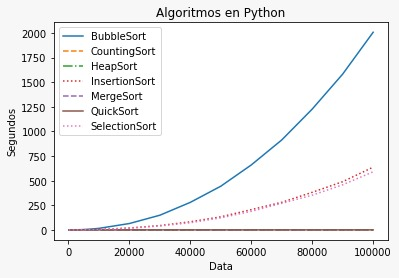
\includegraphics{python.jpeg}\\
        \caption{Figura 8: Comparación de los algoritmos de ordenamiento en Python.}
        \centering
        \end{figure8}\\
        \clearpage
        
  
    \end{enumerate}
	  	
	\end{enumerate}


	
	%\clearpage
	%\bibliographystyle{apalike}
	%\bibliographystyle{IEEEtranN}
	%\bibliography{bibliography}
	
	


		
	
\end{document}

